% -*- Mode: latex; -*-
% $HeadURL: https://outreach.scidac.gov/svn/hpctoolkit/trunk/doc/manual/hpcviewer.tex $
% $Id: hpcviewer.tex 3336 2011-01-03 23:29:25Z tallent $


\HPCToolkit{} provides the \hpctraceviewer{}~\cite{Tallent-MC-etal:2011:hpctoolkit-scalable-tracing} performance presentation tool for interactive examination of performance-trace databases.
\hpctraceviewer{} interactively presents a large-scale trace without concern for the scale of parallelism it represents.


% ===========================================================================
% ===========================================================================

\section{Launching}

\hpctraceviewer{} can either be launched from a command line (Linux/Unix platform) or by clicking the \hpctraceviewer{} icon (for Windows, Mac OS X and Linux/Unix platform).
The command line syntax is as follows:
\begin{quote}
\begin{verbatim}
  hpctraceviewer [options] [<hpctoolkit-database>]
\end{verbatim}
\end{quote}
Here, \texttt{<hpctoolkit-database>} is an optional argument to load a database automatically.
Without this argument, \hpctraceviewer{} will prompt for the location of a database.

The possible options are as follows:
\begin{itemize}
 \item \texttt{-n}: Do not display the Callers View.  (Saves memory and time.)

 \item \texttt{-consolelog}: Send log entries to a console in addition to a log file.
   (To get a console window, be sure to use java as the VM instead of javaw.)

 \item \texttt{-debug}: Log additional information about plug-in dependency problems.
\end{itemize}

% ===========================================================================
% ===========================================================================

%% \section{Installing \hpcviewer{}}

%% \subsection{Requirements}
%% \begin{itemize}
%%  \item Java Runtime Environment (JRE) 1.5 or greater.
%%    Use the Sun or IBM version; we have had problems with OpenJDK.

%%  \item On Linux, GTK+ is required.
%% \end{itemize}


%% \subsection{Generic Instructions}
%% \begin{enumerate}
%%   \item Download \hpcviewer{} package that is suitable for your platform from 
%%     \begin{quote}
%%       \url{https://outreach.scidac.gov/frs/?group\_id=22} 
%%     \end{quote}
%%   \item Untar the tarball into a temporary directory (Linux) or an installation directory (Windows and Mac).
%% \end{enumerate}


%% \subsection{Linux-specific Instructions}

%% To install \hpcviewer{} in an \HPCToolkit{} installation, unpack the tarball and execute the following command:
%% \begin{quote}
%% \begin{verbatim}
%%   ./<hpcviewer>/install <install-path>
%% \end{verbatim}
%% \end{quote}
%% Here, \mytt{<hpcviewer>} is the directory created by unpacking the tarball; and 
%% \mytt{<install-path>} is the same directory passed to the \texttt{--prefix} option of \HPCToolkit{}'s \texttt{configure} script.

%% Typically one compiles and installs \HPCToolkit{} before installing \hpcviewer{}, but this is not necessary.
%% Note, however, that if \hpcviewer{} is installed first, the \mytt{install} script will issue a warning and request confirmation.


% ===========================================================================
% ===========================================================================

\section{Views}

\begin{figure}[t]
\centering{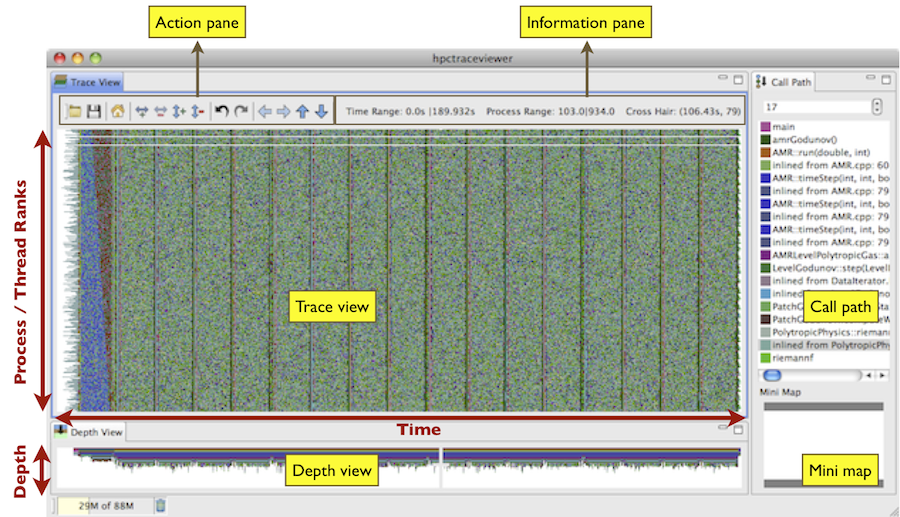
\includegraphics[width=\textwidth]{fig/hpctraceviewer-legend.png}}
\caption{An annotated screenshot of \hpctraceviewer{}'s interface.}
\label{fig:hpctraceviewer-legend}
\end{figure}

Figure~\ref{fig:hpctraceviewer-legend} shows an annotated screenshot of \hpctraceviewer{}'s user interface presenting a call path profile.
The annotations highlight \hpctraceviewer{}'s principal window panes and key controls.
The browser window is divided into three panes.
The Source pane (top) displays program source code.
The Navigation and Metric panes (bottom) associate a table of performance metrics with static or dynamic program structure.


% ===========================================================================
% ===========================================================================

\section{Panes}
\label{sec:hpcviewer:panes}

\hpcviewer{}'s browser window is divided into three panes: the \emph{Navigation pane}, \emph{Source pane}, and the \emph{Metrics pane}.
We briefly describe the role of each pane.

% ===========================================================================
% ===========================================================================

\section{Limitations}

Some important \hpcviewer{} limitations are listed below:
\begin{itemize}

\item \textbf{Limited number of metrics}.
  With a large number of metric columns, \hpcviewer{}'s response time may become sluggish as this requires a large amount of memory.


\end{itemize}
